%-----------------------------------------------------------
% These packages are essential to produce the poster
%-----------------------------------------------------------
\usepackage[scale=1.24]{beamerposter}
\usepackage{graphicx,amsfonts}
\newcounter{figura}
\setcounter{figura}{1}
\usepackage{url}

%-----------------------------------------------------------
% Custom commands that I use frequently
%-----------------------------------------------------------
\newcommand{\bb}[1]{\mathbb{#1}}
\newcommand{\cl}[1]{\mathcal{#1}}
\newcommand{\fA}{\mathfrak{A}}
\newcommand{\fB}{\mathfrak{B}}
\newcommand{\Tr}{{\rm Tr}}
\newtheorem{thm}{Theorem}
\newcommand{\captione}[2]{\begin{minipage}[l]{#1}\begin{center} \textit{Figure \thefigura.}\  #2\end{center}\end{minipage}\addtocounter{figura}{1}}
\newcommand{\spacer}{\begin{column}{\sepwid}\end{column}}
\newcommand{\toplogo}[2]{\newcommand{\posterlogo}{\includegraphics[width=#1]{mypics/#2}}}
\newcommand{\extrainfo}[1]{\newcommand{\inforight}{#1}}
\newcommand{\moreinfo}[1]{\newcommand{\inforightother}{#1}}
\newcommand{\conjetura}[3]{\\[-8mm]\begin{minipage}[l]{30cm}\emph{#1}\end{minipage}& \,\hspace{2cm} \emph{#2}\hspace{2cm}\,\\[-6mm]  \\ \hline}


%-------------------------------------------------------------------------------------------------------------------------------
% These commands will help me to build new blocks, do not modify!
%-------------------------------------------------------------------------------------------------------------------------------

\def\newblock#1#2#3{\expandafter\def\csname Block#1\endcsname{\begin{block}{#2}\rmfamily{#3}\end{block}}}
\def\newAlert#1#2#3{\expandafter\def\csname Alert#1\endcsname{\begin{alertblock}{#2}\rmfamily{#3}\end{alertblock}}}
\def\newSingle#1#2{\expandafter\def\csname Single#1\endcsname{\begin{column}{\onecolwid}#2\end{column}}}
\def\newMarried#1#2{\expandafter\def\csname Married#1\endcsname{\begin{column}{\twocolwid}#2\end{column}}}
\def\newTwin#1#2{\expandafter\def\csname Twin#1\endcsname{\begin{columns}[t,totalwidth=\twocolwid]#2\end{columns}}}

%-----------------------------------------------------------
% Define the column width and poster size
% To set effective sepwid, onecolwid and twocolwid values, first choose how many columns you want and how much separation you want between columns
% The separation I chose is 0.024 and I want 4 columns
% Then set onecolwid to be (1-(4+1)*0.024)/4 = 0.22
% Set twocolwid to be 2*onecolwid + sepwid = 0.464
%-----------------------------------------------------------

\newlength{\sepwid}
\newlength{\onecolwid}
\newlength{\twocolwid}
\setlength{\paperwidth}{48in}
\setlength{\paperheight}{36in}
\setlength{\sepwid}{0.024\paperwidth}
\setlength{\onecolwid}{0.22\paperwidth}
\setlength{\twocolwid}{0.464\paperwidth}
\setlength{\topmargin}{-0.5in}
\usetheme{confposter}

%-----------------------------------------------------------
% Define colours (see beamerthemeconfposter.sty to change these colour definitions)
%-----------------------------------------------------------

\setbeamercolor{block title}{fg=ngreen,bg=white}
\setbeamercolor{block body}{fg=black,bg=white}
\setbeamercolor{block alerted title}{fg=white,bg=dblue!70}
\setbeamercolor{block alerted body}{fg=black,bg=dblue!10}

%-------------------------------
%  START TYPING YOUR BLOCKS !!
%-------------------------------
%%%%  IMPORTANT
%%%%  IMPORTANT
%%%   NO EMPTY ROWS. This example shows what you are NOT to do:
%%%  \newAlert{Main}{Main First Example}{
%%%             This is the main topic, blah blah blah
%%%
%%%             and then blah blah blah
%%%             }
%%

   
\newblock{Introduction}{Introduction}{
    In a recent Ted Talk, pharmacologic adverse events were noted to occur at an unexpectedly higher rate in females than in males. It was suggested that since adverse event rates are often determined by clinical trials, and that clinical trials have an under representation of females, the published adverse event rates may not accurately represent treatment risks for females \cite{TedTalk2}. To determine whether a higher rate of adverse events occurs in females, a large body (over 5 million patient records) of publicly available data published by the FDA were screened \cite{OpenFDA}. The null hypothesis is the proportion of serious adverse event outcome types will be equal for males and females. The alternative hypothesis will be that one of the populations (males or females) will have a higher proportion of one or more serious adverse event outcome types.
}

%%%
\newblock{Definitions}{Definitions}{
  \begin{itemize}
    \item $\beta$-blockers are a class of prescription medication that are indicated for reducing for blood pressure.
    \item Serious Adverse Events include adverse events or suspected adverse reactions when in the view of either the investigator or sponsor, it results in any of the following outcomes: 'Death' (fatal),  'Hospitalization', 'Disabling' 'Congenital Anomali', 'Life Threatening' and 'Other'
  \end{itemize}
}

\newblock{Description}{Adverse Event Description}{
  An adverse event is any unfavorable and unintended sign, symptom, or disease temporarily associated with the use of a drug, without any judgment about causality or relationship to the drug. These events get reported to the FDA along with demographic information about patient. We selected event records where the patient sex was known and the $\beta$-blocker was considered by the reporter to be the primary cause; adverse events where the beta-blocker was concomitant or interacting with another drug were excluded. Each event could be flagged with multiple serious adverse event outcomes.
}

\newblock{Work}{Methods}{
  In a review of data stored at OpenFDA, major drug classes were screened to identify a class where adverse events were common and the number of such events approximated an even distribution between males and females. Of the reviewed classes, $\beta$-blockers met the above inclusion criteria. Within the $\beta$-blocker class of drugs, the following drugs were evaluated: metoprolol, acebutolol, atenolol, nadolol, and bisoprolol. Over 5 million adverse event records were downloaded and inserted into a MongoDB collection. Data was filtered to select adverse events fitting the inclusion criteria. To calculate the statistics, null-distribution and p-value, we followed two-population statistical methods described by Rossman and Chance \cite{Chance}.
}

\newblock{Methods}{Future Work}{
 Given the potential implications to patient safety, additional drug classes and specific drugs should be evaluated using the described technique. Analysis of variance (ANOVA) techniques could be used to further evaluate population sets. Finally these results should be compared with published analyses to verify clinical relevance.
}

\newblock{Conclusions}{Conclusions}{
    This study demonstrated the use of a publicly available big data set to evaluate for statistically significant trends in adverse events between males and females in patients receiving $\beta$-blockers. The study results indicate that a higher proportion of fatal adverse events occurred in women receiving $\beta$-blockers. The study also found a higher proportion of adverse events leading to hospitalizations in men. No significant differences were observed for other serious adverse event outcome types. The use of such analyses to further characterize the safety profiles of pharmacologic therapies using larger data sets outside the clinical trial setting may be clinically useful. 
}

\newblock{Bibliography}{References}{\small
  \begin{thebibliography}{99}
    \bibitem{TedTalk2} McGregor, Alyson, MD. "Why Medicine Often Has Dangerous Side Effects for Women." TEDMED. Providence. Web.
    \bibitem{OpenFDA} U.S. Food and Drug Administration, Drug adverse events, U.S. Department of Health and Human Services; 2018. \url{open.fda.gov/drug/event/}
    \bibitem{Chance} Chance, Beth, Allan Rossman. "Investigating Statistical Concepts,  Applications, and Methods." 2017
  \end{thebibliography}
 }

%%%
\newblock{Acknowledgments}{Acknowledgements}{\small
  We would like to thank the CSUCI mathematics department for their unwavering support. We would also like to thank the open source community for MongoDB, LaTeX, Go, and R.
}

\newblock{Logo}{}{\vspace{-4cm}
      \begin{center}
          
\includegraphics[width=1.2in]{mypics/smily.jpg}
      \end{center}
      }

\newAlert{MainTopic}{Results}{
  \begin{center}
      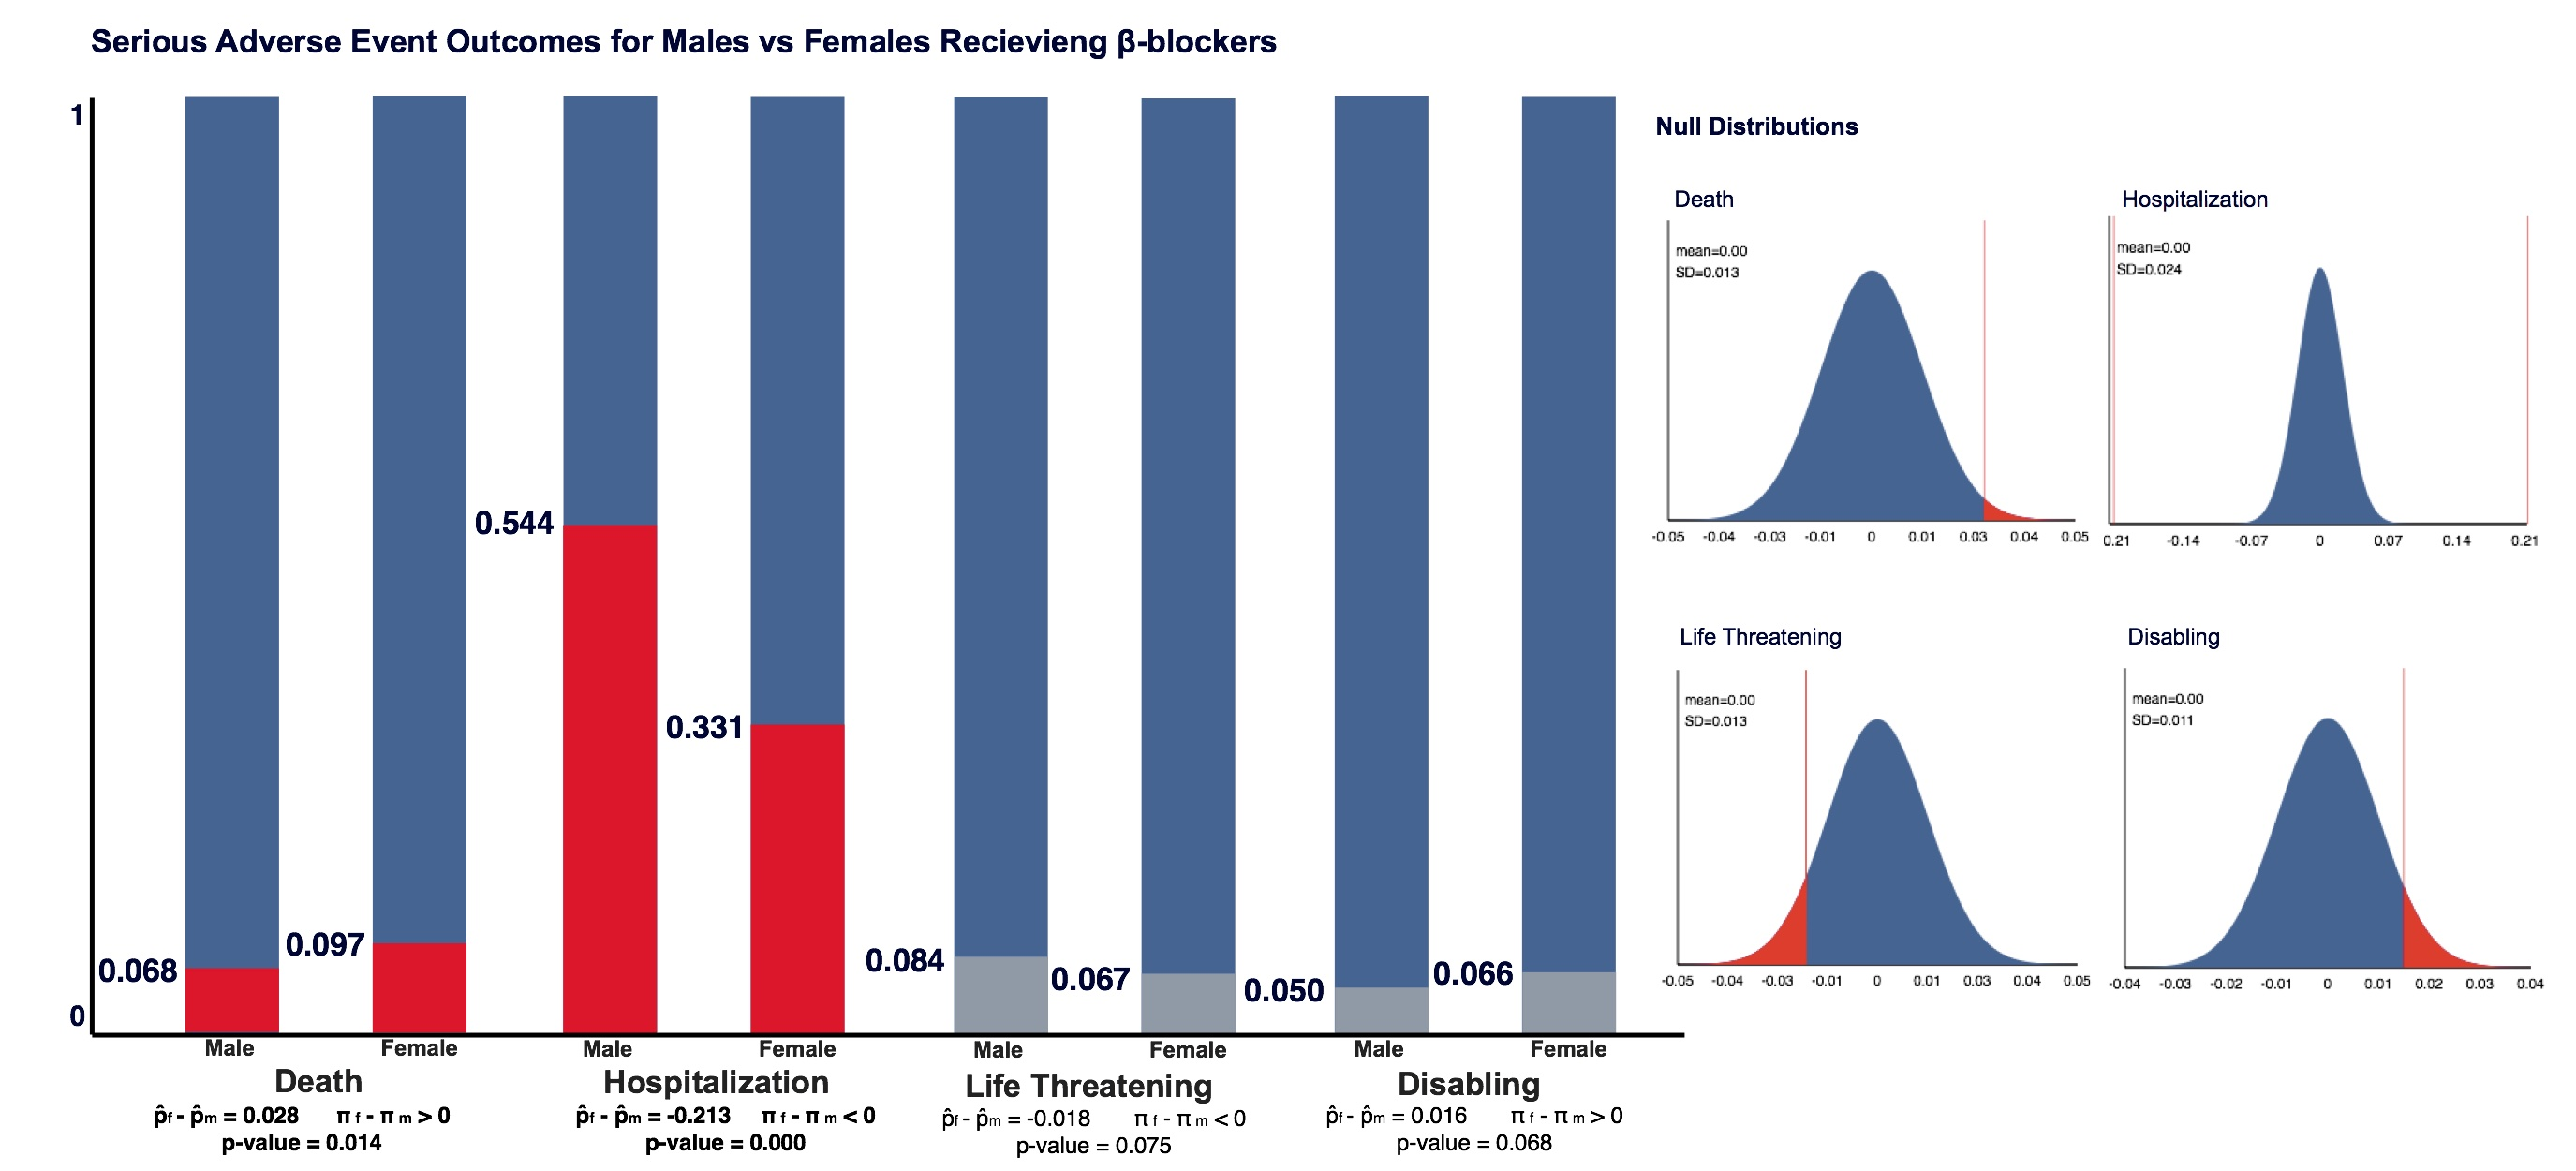
\includegraphics[width=21.5in]{CoolPoster/mypics/posterGraphic.jpg}\hspace{1cm}\\[.2cm]
      \end{center}
}

\newAlert{MainProblem}{Main Problem}{
    The clinical problem is the safety profile of drugs is often based on limited data from clinical trials that may not fully characterize the safety when administered to patients outside of clinical trials (ie, patients in the real world). Real world data sets contain a massive number of records; however, each record may have missing or irrelevant data. The technical problem, in dealing with real world big data, is how to gather, organize, and clean data to efficiently extract valuable information.
}

\newAlert{Conjectures}{Our Hypotheses and P-Values}{
  \begin{tabular}{l l l r}
    \hspace{0.05in}$H_{0}$ & $\pi_{m} = \pi_{f}$ & Male and female populations have no significant difference AE severity. & \hspace{0.05in} \\
    \hspace{0.05in}$H_{a1}$ & $\pi_{m} < \pi_{f}$ & The female population has a greater proportion of \textbf{fatal} AEs. & \textbf{p=0.014} \hspace{0.05in} \\
    \hspace{0.05in}$H_{a2}$ & $\pi_{m} > \pi_{f}$ & The male population has a greater proportion of \textbf{hospitalizing} AEs. & \textbf{p=0.00} \hspace{0.05in} \\
    \hspace{0.05in}$H_{a3}$ & $\pi_{m} > \pi_{f}$ & The male population has a greater proportion of life threatening AEs & p=0.075 \hspace{0.05in} \\
    \hspace{0.05in}$H_{a4}$ & $\pi_{m} < \pi_{f}$ & The female population has a greater proportion of disabling AEs. & p=0.068 \\
  \end{tabular}
}
